% új oszloptípus a tördeléshez
\newcolumntype{Y}{>{\raggedright\arraybackslash}X}


\Chapter{Koncepció}

\Section{Tartalom és felépítés}

Ebben a fejezetben a dolgozat témáját körülhatároljuk, bemutatjuk a releváns projektmenedzsment rendszereket, azok főbb funkcióit, előnyeit és hátrányait, valamint azt, hogyan kapcsolódnak az Acxor fejlesztéséhez. A cél nem a saját eredmények részletezése, hanem egy átfogó, irodalmi és technológiai alap bemutatása, amelyre a dolgozat további részei építenek. A fejezet négy fő területre koncentrál: irodalomkutatás, technológia, piackutatás és követelmény-specifikáció. Az irodalomkutatás során áttekintjük a legfontosabb projektmenedzsment rendszereket, a technológiai részben bemutatjuk a rendszerek főbb funkcióit, a piackutatás során összehasonlítjuk a meglévő megoldásokat, míg a követelmény-specifikációban az Acxor fejlesztés céljait és alapelveit foglaljuk össze.

\Section{Projektmenedzsment rendszerek áttekintése}

\SubSection{JIRA}

A JIRA egy komplex, vállalati szintű projektmenedzsment és issue tracking rendszer. Kiemelt jellemzői \cite{jira}:

\begin{itemize}
\item issue tracking, Agile metodikák (Scrum / Kanban) támogatása,
\item workflow testreszabás,
\item jogosultságkezelés,
\item riportok és dashboardok,
\item széleskörű integrációk (Confluence, Bitbucket, GitHub, Slack, Teams).
\end{itemize}

A JIRA rugalmas és szinte bármi testreszabható, ami előnyt jelent nagyvállalati környezetben, ugyanakkor komplexitása miatt tanulási görbéje meredek. A rendszer hierarchiája Epic–Story–Task–Subtask struktúrát követ, ami előnyös a nagy csapatok számára. Automatizmusai trigger–condition–action logikán alapulnak, amely lehetővé teszi például automatikus állapotváltást, assignee hozzárendelést, vagy e-mail értesítések küldését.

Az Acxor fejlesztésében a JIRA inspirációként szolgált a funkcionalitás és a workflow kezelés terén, de egyszerűsített felhasználói felületet és átláthatóbb jogosultsági modellt alkalmaz. A felület a \ref{fig:jira}. ábrán látható.

\begin{figure}[h!]
\centering
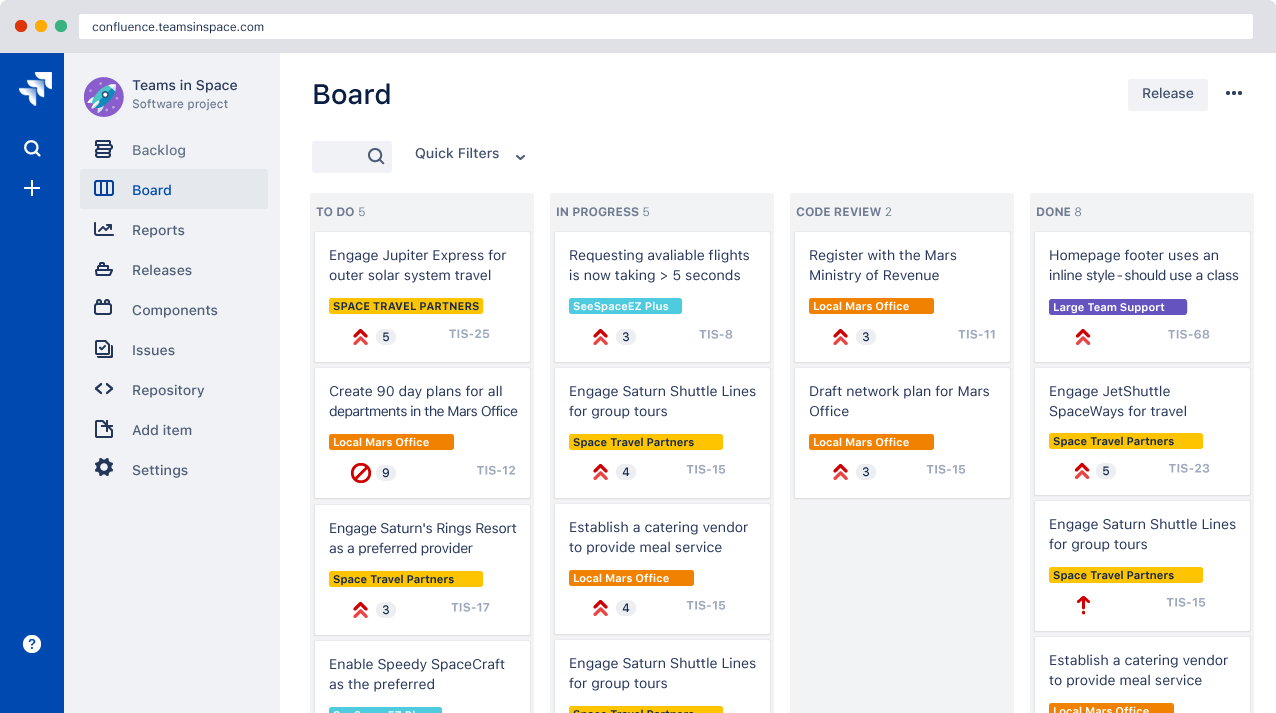
\includegraphics[width=0.75\textwidth]{images/jira.png}
\caption{A Jira sprint- és issue-kezelő felülete \cite{jira}}
\label{fig:jira}
\end{figure}

\SubSection{Trello}

A Trello egy intuitív, kártya-alapú projektmenedzsment rendszer, amely kisebb csapatoknak vagy egyszerűbb folyamatokhoz ideális. Főbb jellemzői \cite{trello}:

\begin{itemize}
\item Board → List → Card → Checklist vizuális hierarchia,
\item drag \& drop alapú kezelés,
\item minimális konfiguráció és real-time szinkron,
\item egyszerű automatizmusok (Butler).
\end{itemize}

A Trello előnye a gyors betanulás és a vizuális, átlátható felület, míg hátránya a korlátozott testreszabhatóság és a nagyobb projektekhez kevésbé megfelelő komplexitás. Az Acxor esetében a Trello inspirálta az intuitív, vizuális task lifecycle és board kezelést, amely egyszerre egyszerű és professzionális. A felület a \ref{fig:trello}. ábrán látható.

\begin{figure}[h!]
\centering
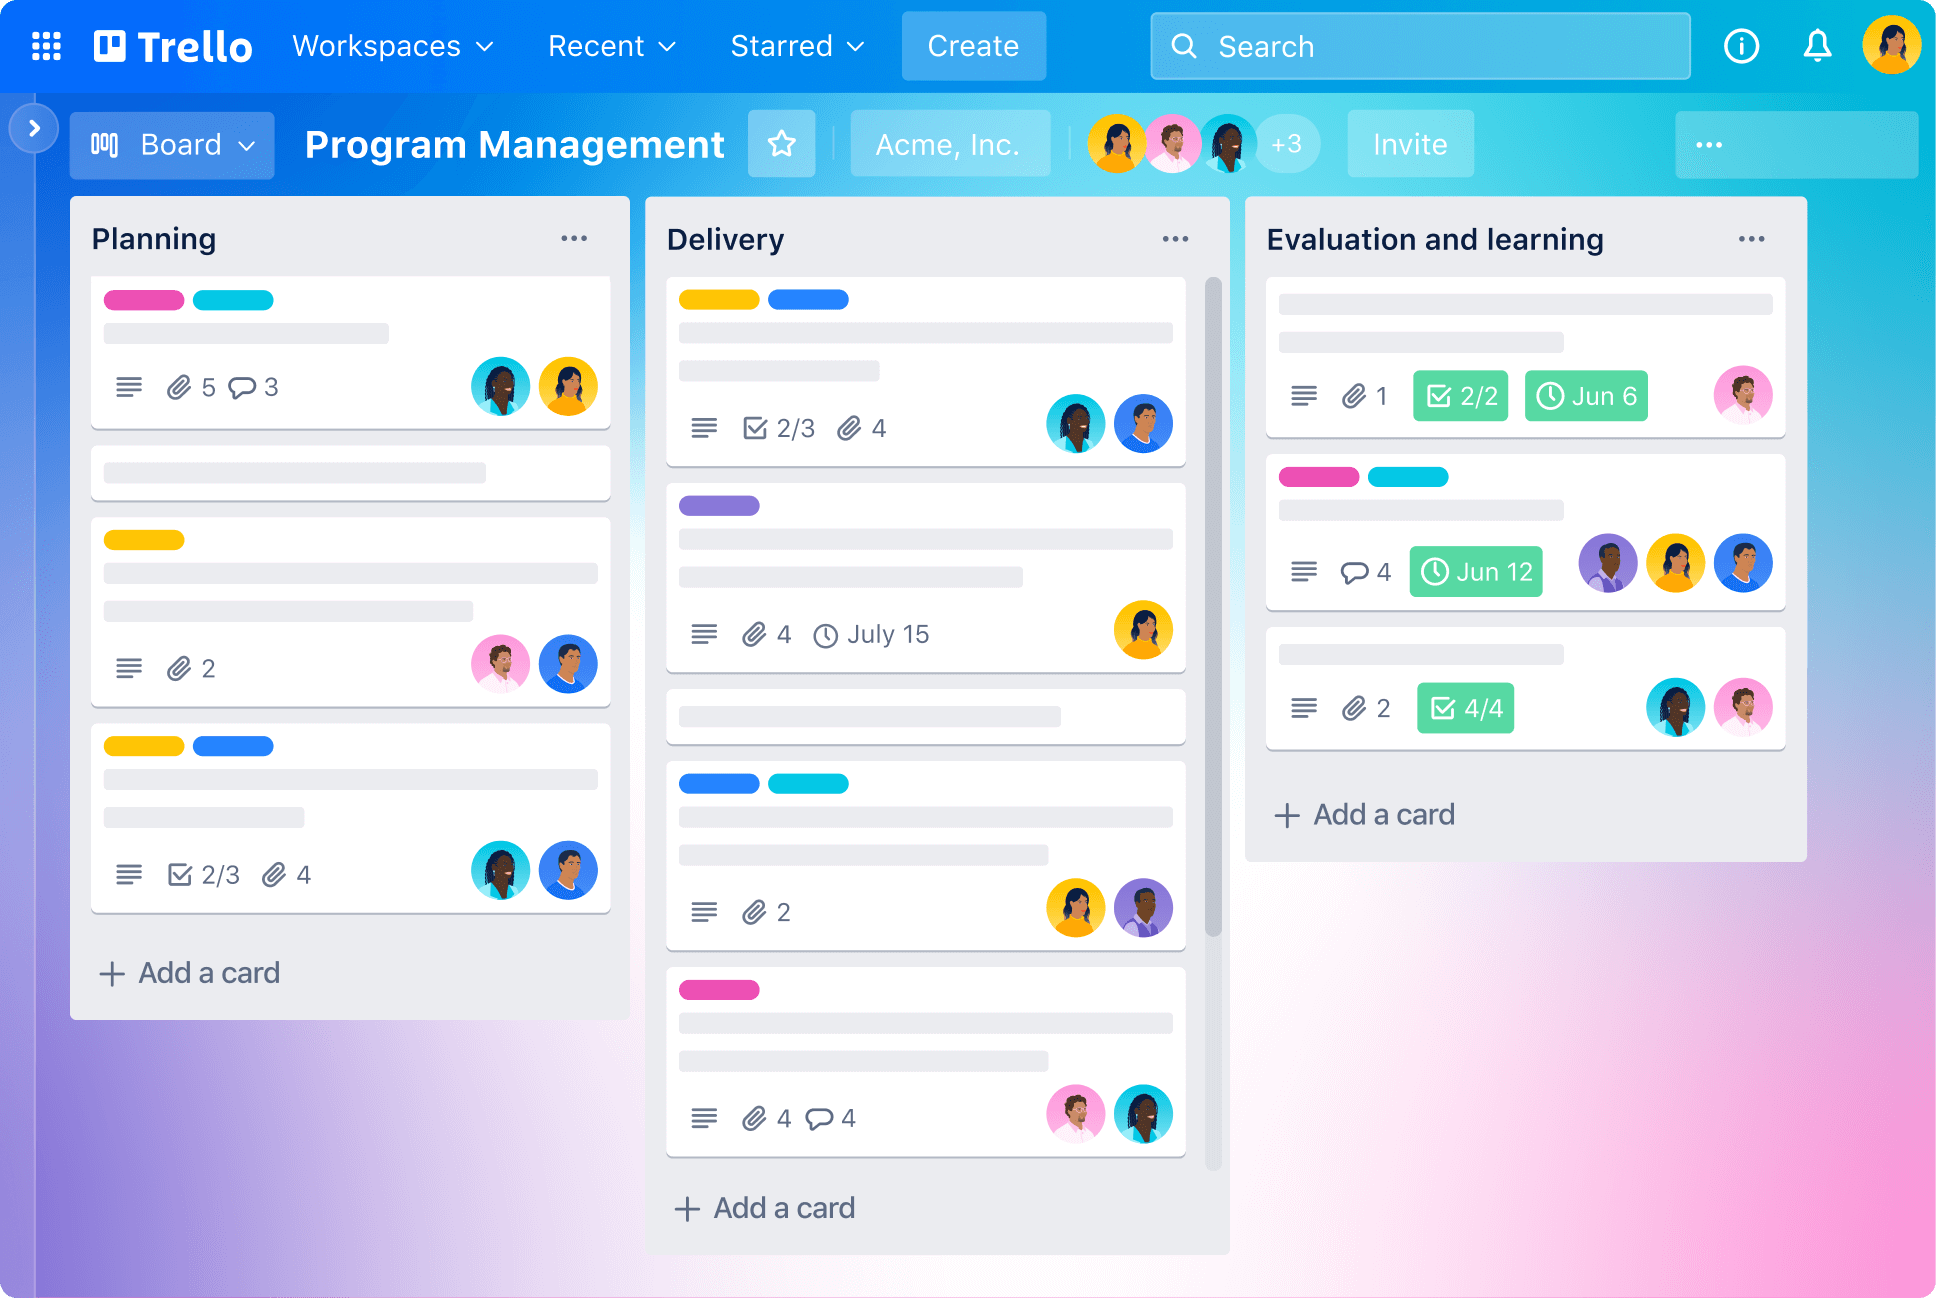
\includegraphics[width=0.8\textwidth]{images/trello.png}
\caption{A Trello Kanban-alapú feladatkezelő felülete \cite{trello}}
\label{fig:trello}
\end{figure}

\SubSection{Asana}

Az Asana egy feladat- és projektmenedzsment platform, amely a csapatok együttműködését támogatja. Fő funkciói \cite{asana}:

\begin{itemize}
\item task és subtask kezelés,
\item projektek és Timeline vizualizáció,
\item határidők és felelősök hozzárendelése,
\item dashboard és riporting,
\item integráció külső szolgáltatásokkal (Slack, Teams, GitHub, Google Workspace).
\end{itemize}

Előnye a könnyen átlátható felület és a gyors onboarding, hátránya a korlátozott workflow testreszabás és a részletes riporting hiánya. Az Acxor tervezésénél az Asana inspirációt jelentett a fókuszált task lifecycle és minimalista felület kialakításában. A felület a \ref{fig:asana}. ábrán látható.

\begin{figure}[h!]
\centering
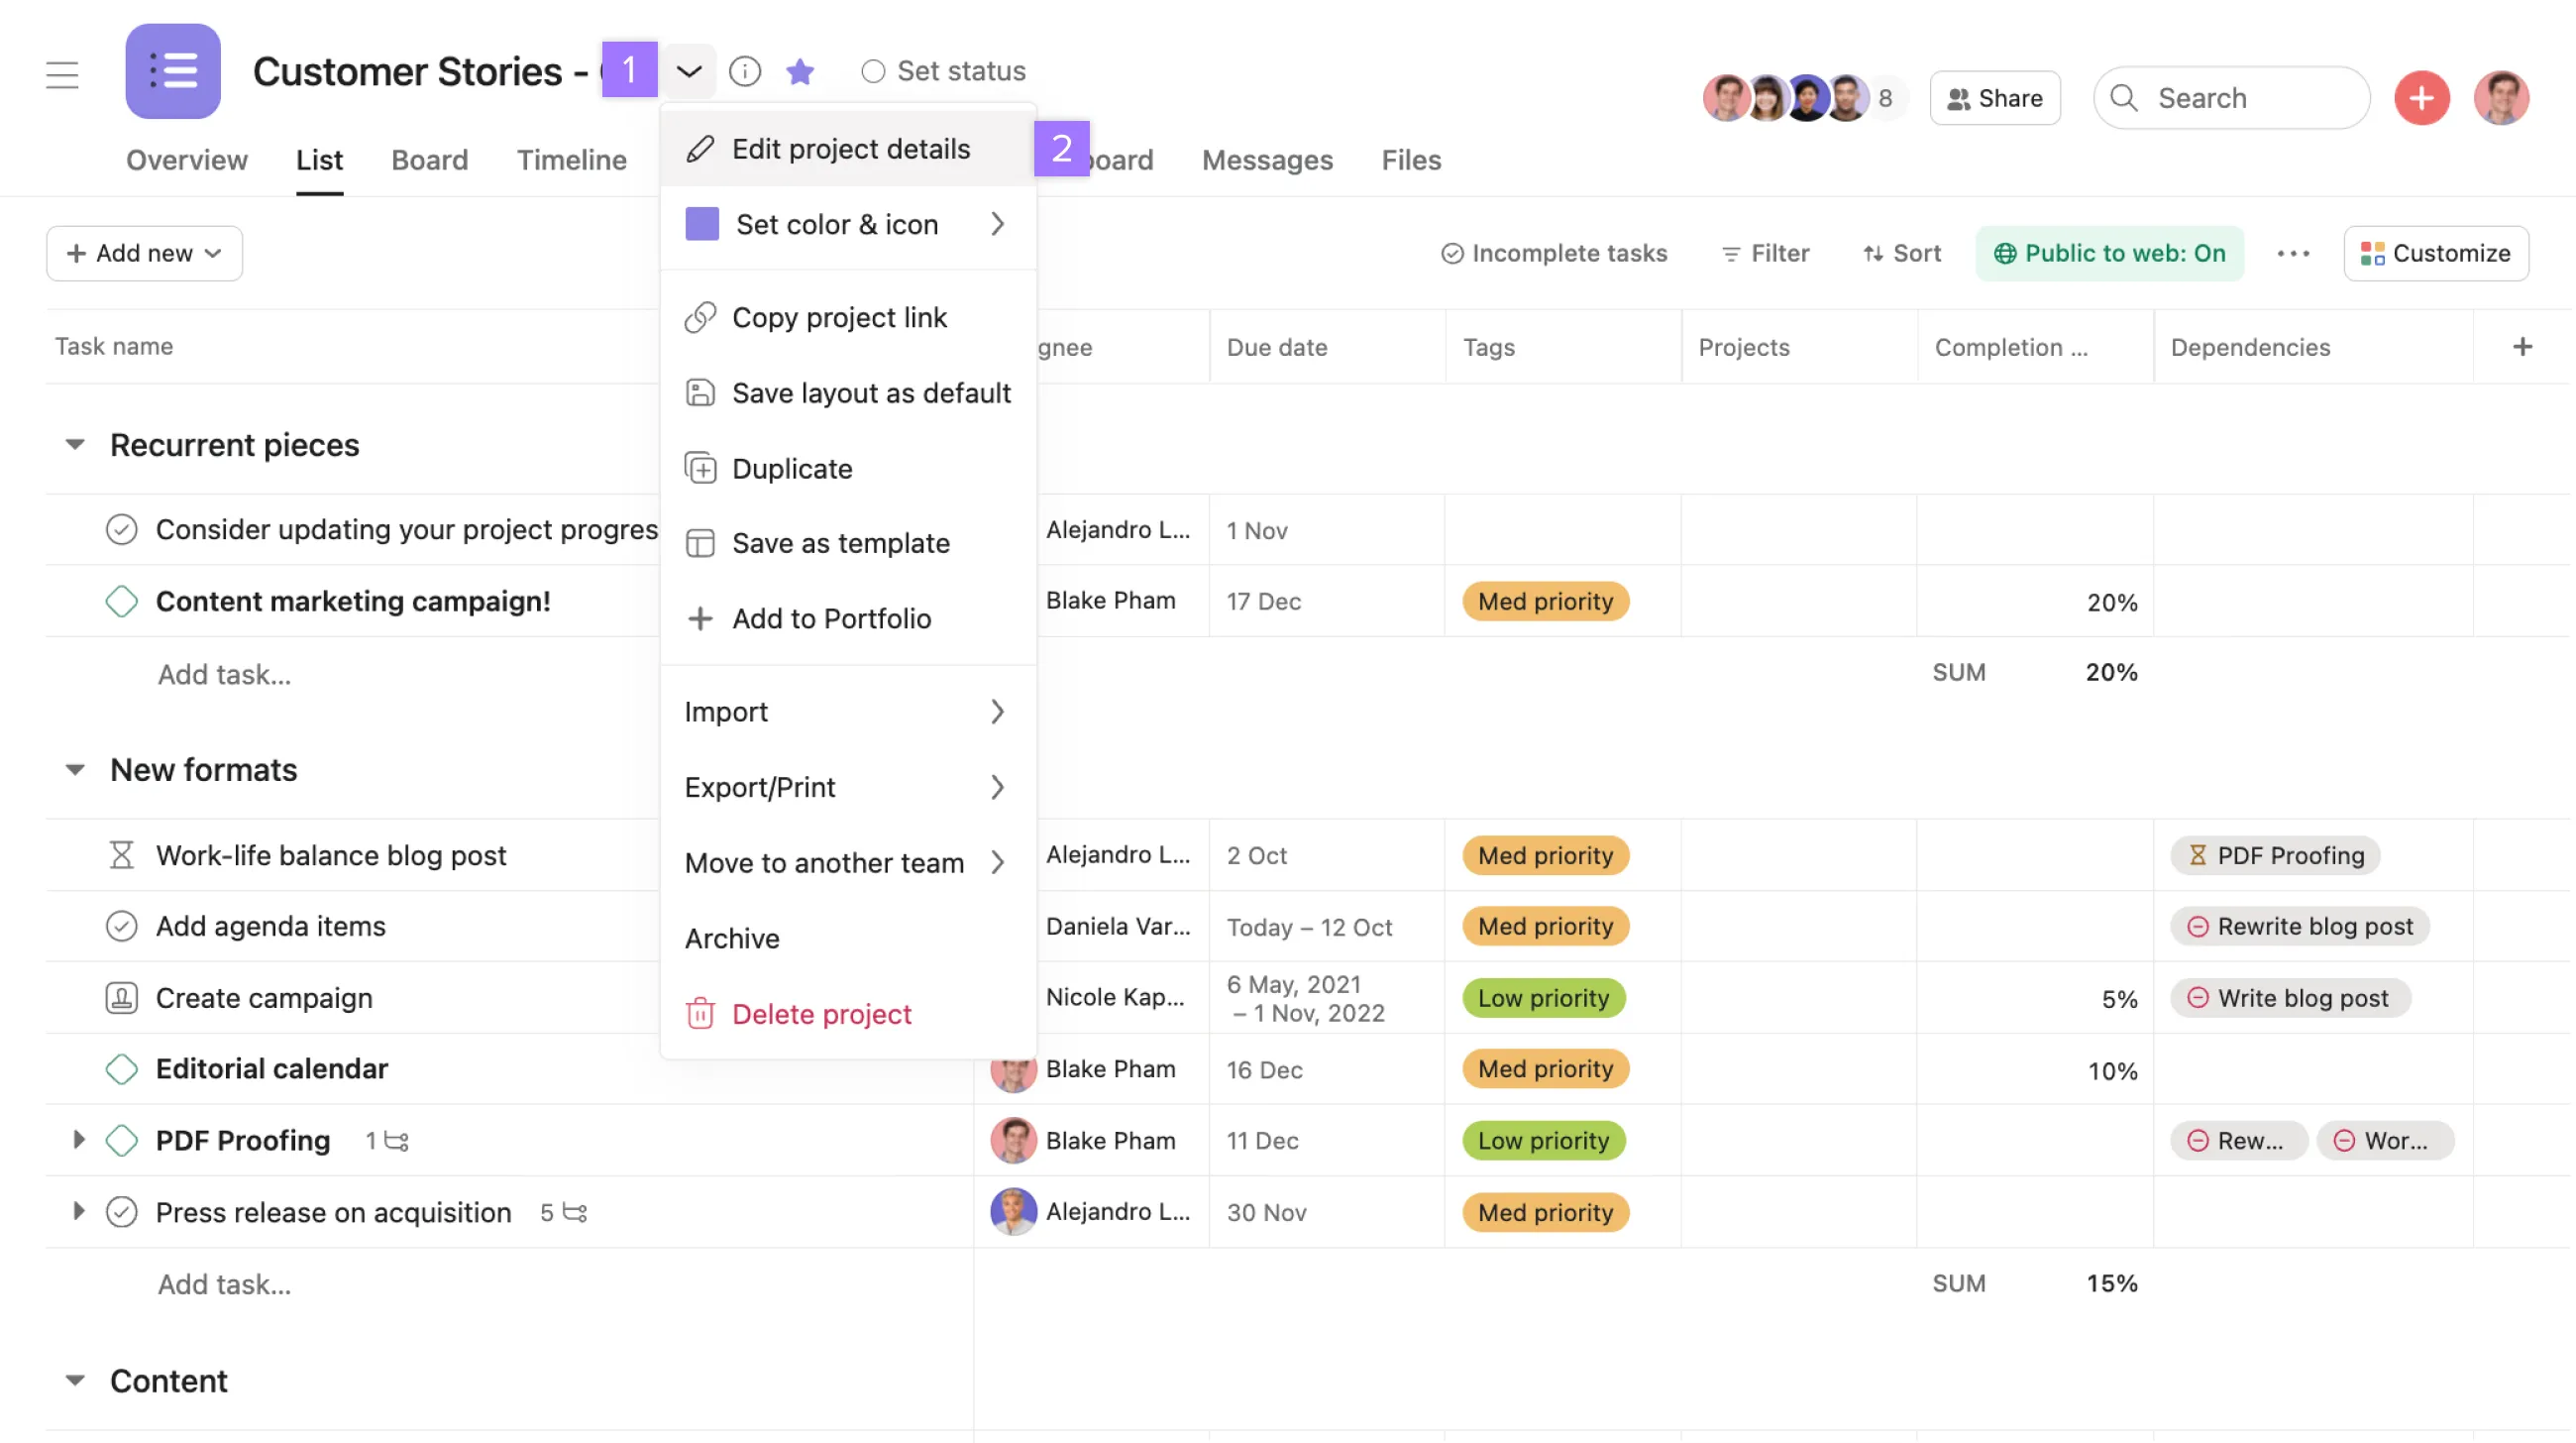
\includegraphics[width=0.8\textwidth]{images/asana.png}
\caption{Az Asana projektmenedzsment eszköz felülete \cite{asana}}
\label{fig:asana}
\end{figure}

\SubSection{Redmine}

A Redmine nyílt forráskódú rendszer, amely elsősorban testreszabhatóságáról és bővíthetőségéről ismert. Főbb jellemzői \cite{redmine}:

\begin{itemize}
\item issue tracking és projekt hierarchia (főprojekt → alprojekt),
\item testreszabható workflow és permission rendszer,
\item Gantt és Calendar vizualizáció,
\item plugin és API alapú integráció.
\end{itemize}

Előnye a nagy projektek kezelésére való alkalmasság és a nyílt forráskódú bővíthetőség, míg hátránya a kevésbé modern UI és a tanulási görbe. Az Acxorban a Redmine inspirációt jelentett a backend struktúrában és az issue hierarchia egyszerűsítésében, modern, letisztult felülettel. A felület a \ref{fig:redmine}. ábrán látható.

\begin{figure}[h!]
\centering
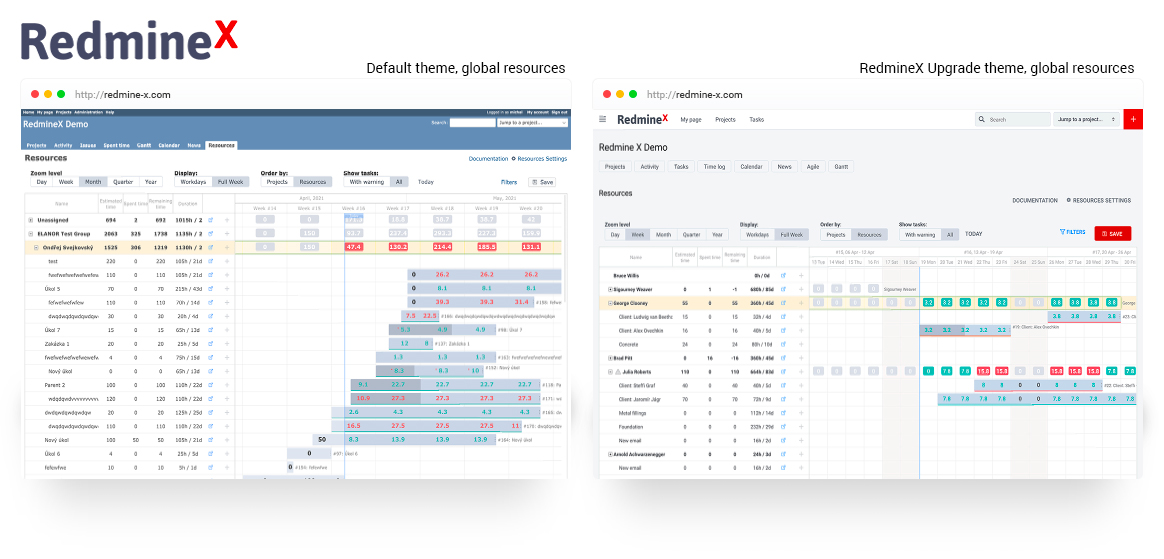
\includegraphics[width=0.8\textwidth]{images/redmine.jpg}
\caption{A Redmine nyílt forráskódú projektmenedzsment eszköz felülete \cite{redmine}}
\label{fig:redmine}
\end{figure}

\SubSection{Projektmenedzsment rendszerek összehasonlítása}

Az Acxor a közepes komplexitású fejlesztői csapatok számára készült, kiemelten figyelve a vizualitásra, egyszerűségre és motivációs rendszerekre. A \ref{tab:comparison1}. és \ref{tab:comparison2}. táblázat összehasonlítja az Acxort a Trello-val és a Jira-val, illetve a Redmine-nel és az Asana-val.

\begin{table}[h!]
\centering
\scriptsize
\setlength{\arrayrulewidth}{0.5pt}
\begin{tabularx}{\textwidth}{|l|Y|Y|Y|}
\hline
\textbf{Funkció / Eszköz} & \textbf{Acxor} & \textbf{Trello} & \textbf{Jira} \\
\hline
Webes felület & Modern vizuális UI & Webes, vizuális & Webes, komplex \\
Kanban board & Beépített, drag\&drop & Beépített & Részben, plugin szükséges \\
Sprint / Iteration & Részben, egyszerű & -- & Teljes körű \\
Gamifikáció & XP, szint, badge & -- & -- \\
Task / Subtask & \makecell[l]{Epic $\rightarrow$ Story \\ Task $\rightarrow$ Subtask} & Kártya / checklist & \makecell[l]{Epic $\rightarrow$ Story \\ Task $\rightarrow$ Subtask} \\
Chat / Log & Globális bot & Részben, kommentek & Részben, jegy alapú \\
Workflow testreszabás & Részben, egyszerű & Részben, limitált & Részletes, szabály alapú \\
Permission rendszer & Részben, egyszerű & Részben, egyszerű & Mély, szerepkör alapú \\
Integrációk & Alap, kulcs szolgáltatások & Részben, Power-Ups & Széles (Confluence, GitHub, Slack\ldots) \\
\hline
\end{tabularx}
\caption{Acxor összehasonlítása a Trello-val és a Jira-val \cite{trello, jira}}
\label{tab:comparison1}
\end{table}

\begin{table}[h!]
\centering
\scriptsize
\setlength{\arrayrulewidth}{0.5pt}
\begin{tabularx}{\textwidth}{|l|Y|Y|Y|}
\hline
\textbf{Funkció / Eszköz} & \textbf{Acxor} & \textbf{Redmine} & \textbf{Asana} \\
\hline
Webes felület & Modern vizuális UI & Webes, részletes & Webes, intuitív \\
Kanban board & Beépített & Részben, plugin szükséges & Board / list nézet \\
Sprint / Iteration & Részben, egyszerű & Teljes körű & Részben, idővonal / Timeline \\
Gamifikáció & XP, szint, badge & -- & -- \\
Task / Subtask & Egyszerű hierarchia & Issue / subtask & Task / subtask \\
Chat / Log & Globális bot & Részben, jegy alapú & Részben, kommentek \\
Workflow testreszabás & Részben, egyszerű & Részletes & Részben, egyszerű \\
Permission rendszer & Részben, egyszerű & Roles alapú & Részben, alap \\
Integrációk & Kulcs szolgáltatások & Részben, pluginok, SCM & Slack, GitHub, Google Workspace \\
\hline
\end{tabularx}
\caption{Acxor összehasonlítása a Redmine-nel és az Asana-val \cite{redmine, asana}}
\label{tab:comparison2}
\end{table}

A fenti rendszerek áttekintése rávilágít arra, hogy a projektmenedzsment eszközök széles skálán helyezkednek el komplexitás, testreszabhatóság és felhasználói élmény szempontjából. Az Acxor célja a különböző rendszerek előnyeinek ötvözése: a JIRA funkcionalitásának, a Trello vizuális egyszerűségének, az Asana átlátható task lifecycle-jának, valamint a Redmine struktúrájának kombinálása egy intuitív, könnyen használható, ugyanakkor professzionális projektmenedzsment platformban.

Ez a koncepciói alap biztosítja, hogy a dolgozat későbbi fejezeteiben bemutatott fejlesztések jól meghatározott, átgondolt irányelv szerint történjenek, és az olvasó számára érthető, követhető legyen a választott megközelítés és technológiai háttér.